
\documentclass{article}
\usepackage[utf8]{inputenc}
\usepackage[sexy]{evan}
\usepackage{framed}
\usepackage{amsmath}
\usepackage{float}
\DeclareMathOperator\Arg{Arg}
\DeclareMathOperator{\arcsec}{arcsec}
\DeclareMathOperator{\arccot}{arccot}
\DeclareMathOperator{\arccsc}{arccsc}
\DeclareMathOperator{\trig}{trig}
\DeclareMathOperator{\arctrig}{arctrig}
\usepackage{array}

\title{Trigonometry With Tears}
\author{aSquaredRush}
\date{}

\begin{document}
\maketitle
\tableofcontents
\newpage



\section{Basics}
\noindent We start by defining $\sin(\theta)$ and $\cos(\theta)$. On a unit circle, $x=\cos(\theta)$ and $y=\sin(\theta)$. From here, we can derive the periods of both functions as well. The $x,y$ values repeat every rotation around the circle($2\pi$ radians). 
\vspace{5mm}

\noindent We can then also define $\tan(\theta)$ as the ratio between $\sin(\theta)$ and $\cos(\theta)$. We can see that due to the signs of $x,y$, the period of tangent is $\pi$ radians. 

\vspace{5mm}

\subsection{Period, Amplitude, Phase Shift, Vertical Shift}
\noindent The period of a function $\trig(\theta$ is an angle $\alpha$ such that $trig(\theta+\alpha)$ = $trig(\theta)$. This means that even though 2$\pi$ is a period of $\sin$, 4$\pi$ also is. This applies for any integer multiple of 2$\pi$. From here on out, the period of a function refers to the primitive period, i.e. the lowest positive period of a function. This applies to all MAO tests as well.

\vspace{5mm}
\noindent The amplitude can be thought of as the maximum value of a trigonometric function centered on the y-axis at 0(I know it's a bit wonky, but who cares- I'll explain more later). Notice that tangent has no amplitude. Any other trig functions that don't have a maximum or minimum also have no amplitude.

\vspace{5mm}
\noindent The phase shift and vertical shift represent how much of an x or y translation the function has. 

\subsection{General Trigonometric Function}
$$a\trig{(bx+c)}+d$$ 
is the general formula for a trigonometric function where $a$ is the amplitude, $\frac{-c}{b}$ is the phase shift, $d$ is the vertical shift, and the period is $\frac{\textrm{The normal period}}{b}$. 

\vspace{5mm}
\noindent For the period, this makes sense because a large value of $b$ means a very compressed function and a small period and vice versa.

\vspace{5mm}
\noindent Because the phase shift represents how far from 0 the function has shifted on the x-axis, we need a $x-\_$ term. If we factor out $b$ in the argument of the function, we get $b(x+c/b)$, and this is clearly shifted $\frac{-c}{b}$ from 0. 

\vspace{5mm}
\noindent The amplitude just affects the maximum or minimum of the function. $a\sin(x)$ has a maximum and minimum of $a$ and $-a$.

\pagebreak
\subsection{Functions}
\begin{definition}
[The basic trigonometric functions]

$$\sin(\theta) \textrm{ and } \arcsin(\alpha)$$


$$\cos(\theta) \textrm{ and } \arccos(\alpha)$$


$$\tan(\theta) \textrm{ and } \arctan(\alpha)$$


$$\csc(\theta) = \frac{1}{\sin(\theta)} \textrm{ and } \arccsc(\alpha)$$


$$\sec{}(\theta) = \frac{1}{\sin(\theta)} \textrm{ and } \arcsec(\alpha)$$


$$\csc(\theta) = \frac{1}{\cos(\theta)} \textrm{ and } \arccsc(\alpha)$$


$$\cot(\theta) = \frac{1}{\tan(\theta)} = \frac{\cos(\theta)}{\sin(\theta)} \textrm{ and } \arccot(\alpha)$$



$$\textrm{Where } \trig{\theta} = \alpha \textrm{ and } \arctrig{\alpha} = \theta$$

\end{definition}

\noindent The arc-functions give you the angle back from the trig function.

\vspace{5mm}
\noindent The arc-functions have limitations on their ranges, so they can be functions. Let's take $\arcsin(\alpha)$, for example. If you wanted $\arcsin(\frac{1}{2})$, what angle would you get back? $30^{\circ}$ or $150^{\circ}$? To get only one value, we restrict the range of $\arcsin$ to be $[-\frac{\pi}{2},\frac{\pi}{2}]$



\pagebreak
\section{Identities and Formulas}

These are the essential formulas. Almost all others can be derived from these:



\begin{theorem}
\noindent $\sin(\theta)^2+\cos(\theta)^2=1$ due to the Pythagorean Theorem using legs of a right triangle in a unit circle.

\vspace{5mm}
\noindent $1+\tan(\theta)^2=\sec(\theta)$. This can be proved by writing $\tan(\theta)$ and $\sec(\theta)$ in terms of $\sin(\theta)$ and $\cos(\theta)$. 

\vspace{5mm}
\noindent $1+\cot(\theta)^2=\csc(\theta)^2.$ This can be proved by writing $\cot(\theta)$ and $\csc(\theta)$ in terms of $\sin(\theta)$ and $\cos(\theta)$.
\end{theorem}

\subsection{Angle Sum/Difference Formulas}

Let's start off by going away from trigonometry for a second, and use complex numbers. Any complex number can be represented by $r$cis$(\theta)=r(\cos(\theta)+i\sin(\theta))$ We can notice that this looks very similar to a Cartesian coordinate in the form of (x,y), but instead, this is in the form of $(\cos(\theta),\sin(\theta))$ The $r$ isn't needed because $\sin(\theta)$ and $\cos(\theta)$ have a maximum value of 1. 

\vspace{5mm}
\noindent There is a geometric proof for the angle sum identities, but the complex proof is much simpler(pun intended). Using the properties of complex numbers, we know cis$(\theta+\alpha) = $cis$(\theta)$cis$(\alpha)$. 

\vspace{5mm}
\noindent Rewriting the cis's in terms of $\sin$ and $\cos$ gives cis$(\theta+\alpha) = (\cos(\theta)+i\sin(\theta))(\cos(\alpha)+i\sin(\alpha))$. Expanding gives us $\cos(\theta)\cos(\alpha)-\sin(\theta)\sin(\alpha)+i(\sin(\theta)\cos(\alpha)+\cos(\theta)\sin(\alpha))$  

\vspace{5mm}
\noindent Because cis$(\theta+\alpha) = \cos(\theta+\alpha)+i\sin(\theta+\alpha)$, we can equate the real and imaginary terms of the expansion with this to get $$\cos(\theta+\alpha) = \cos(\theta)\cos(\alpha)-\sin(\theta)\sin(\alpha)$$ and $$\sin(\theta+\alpha) = \sin(\theta)\cos(\alpha)+\cos(\theta)\sin(\alpha)$$ Finding the difference is just plugging in $-\alpha$ and using the even and odd properties of $\cos$ and $\sin$, respectively.

\vspace{5mm}
\noindent This might seem like a lot of work, but it's really easy to remember and derive by hand compared to seeing it in this pdf.

\vspace{5mm}
\pagebreak
\noindent You might recall that tangent is the ratio of sine to cosine. So,
\begin{align*}
\tan(\alpha + \theta) &= \frac{\sin( \theta \pm \alpha)}{\cos(\theta \pm \alpha)} \\
&= \frac{\sin(\theta) \cos(\alpha) \pm \cos(\theta) \sin(\alpha)}{\cos(\theta) \cos(\alpha) \mp \sin(\theta) \sin(\alpha)} \\
&= \frac{\frac{1}{\cos(\theta)\cos(\alpha)}}{\frac{1}{\cos(\theta)\cos(\alpha)}} * \frac{\sin(\theta) \cos(\alpha) \pm \cos(\theta) \sin(\alpha)}{\cos(\theta) \cos(\alpha) \mp \sin(\theta) \sin(\alpha)} \\
&= \frac{\tan(\alpha)\pm\tan(\theta)}{1\mp\tan(\alpha)\tan(\theta)}
\end{align*}





\vspace{5mm}
\begin{theorem}
[Sum/Difference Formulas]


\vspace{5mm}
\noindent $$\cos(\theta\pm\alpha) = \cos(\theta)\cos(\alpha)\mp\sin(\theta)\sin(\alpha)$$

\vspace{5mm}
\noindent $$\sin(\theta\pm\alpha) = \sin(\theta)\cos(\alpha)\pm\cos(\theta)\sin(\alpha)$$

\vspace{5mm}
\noindent $$\tan(\alpha\pm\theta) = \frac{\tan(\alpha)\pm\tan(\theta)}{1\mp\tan(\alpha)\tan(\theta)}$$


\end{theorem}



\subsection{Double Angle, Triple Angle.....}
\noindent To continue the theme of complex numbers in trigonometry, let me show you a \textit{much} quicker way of deriving multiples of angles. 

\vspace{5mm}
\noindent We know cis$(A)$ represents a complex number. cis$(A)^n = $cis$(nA)$. In other words $(\cos(A)+i\sin(A))^n=\cos(nA)+i\sin(nA)$. Well,  $(\cos(A)+i\sin(A))$ can be represented as $x+iy$. Raising this to the $n'th$ power is the same thing as $(x+y)^n$ but with a slight twist. 

\vspace{5mm}
\noindent First, we know $(x+y)^n$ can be represented through Pascal's Triangle. The coefficients of $(x+y)^n$ are the coefficients of the $n'th$ row of Pascal's Triangle. Keep in mind that the first row is the 0th row. 

\vspace{5mm}
\noindent Now, we're faced with a problem. We need $(x+iy)^n$, but Pascal's Triangle only covers $(x+y)^n$. This can be solved. By the Binomial Theorem, for the first element of the nth row of Pascal's Triangle, the exponent of $iy$ is 0. For the second element, it's 1, for the third, it's 2, and for the fourth it's 3... This means the coefficient of the first element in the nth row is real while the second element is not, the third element is, and the fourth element is not... We also know that the nth row of Pascal's Triangle is equal to $\cos(nA)+i\sin(nA)$. This means we can equate the real and imaginary parts of the nth row of Pascal's Triangle with $\cos(nA)+i\sin(nA)$. From this we get $\cos(nA) = $ the odd indexed elements of the nth row of Pascal's Triangle while $\sin(nA) = $ the even indexed elements of the nth row of Pascal's Triangle.

\vspace{5mm}
\noindent If you managed to make it through that wall of text, but you are still a bit confused, here is an example problem: find $\cos(4x)$ in terms of $\cos(x)$. Well, we know that the 4th row of Pascal's Triangle is 1 4 6 4 1 which means we want 1,6, and 1 as they are the odd indexed elements. By the Binomial Theorem, this is $\cos(x)^4, {4\choose2} \cos(x)^2\sin(x)^2,$ and $\sin(x)^4$. By our Pythagorean Identities, we know $\sin(x)^2 = 1-\cos(x)^2$, and we also know $\sin(x)^4=(\sin(x)^2)^2=(1-\cos(x)^2)^2$, so the final answer should become clear after some substitution.

\vspace{5mm}


\subsubsection{Using Complex Pascal's Triangle to Find n-angle formulas}
\vspace{5mm}
\makebox[\linewidth]{
\begin{tabular}{rccccccccccccccccccc}
&    &    &    &    &    &    &    &    &  1\\\noalign{\smallskip\smallskip}
&    &    &    &    &    &    &    &  1 &    &  1i\\\noalign{\smallskip\smallskip}
&    &    &    &    &    &    &  1 &    &  2i &    &  -1\\\noalign{\smallskip\smallskip}
&    &    &    &    &    &  1 &    &  3i &    &  -3 &    &  -1i\\\noalign{\smallskip\smallskip}
&    &    &    &    &  1 &    &  4i &    &  -6 &    &  -4i &    &  1\\\noalign{\smallskip\smallskip}
&    &    &    &  1 &    &  5i &    & -10 &    & -10i &    &  5 &    &  1i\\\noalign{\smallskip\smallskip}
&    &    &  1 &    &  6i &    & -15 &    & -20i &    & 15 &    &  6i &    &  -1\\\noalign{\smallskip\smallskip}
&    &  1 &    &  7i &    & -21 &    & -35i &    & 35 &    & 21i &    &  -7 &    &  -1i\\\noalign{\smallskip\smallskip}
&  1 &    &  8i &    & -28 &    & -56i &    & 70 &    & 56i &    & -28 &    &  -8i &    &  1\\\noalign{\smallskip\smallskip}
1 &    &  9i &    & -36 &    & -84i &    & 126 &    & 126i &    & -84 &    & -36i &    &  9 &    &  1i\\\noalign{\smallskip\smallskip}
\end{tabular}
}

\vspace{5mm}
\noindent This triangle \textbf{should not} be memorized; rather, learn Pascal's Triangle and its relation to binomial theorem. Every other element has an $i$ term because of how $i^k$ alternates in the binomial expansion of $(x+iy)^n$. This is also why some terms are negative $i^2=-1$ and $i^3=-i$.

\begin{example}
\begin{problem}
Find $\cos(4\theta)$ in terms of only $\sin$;
\end{problem}


\noindent Remember that in the expansion of $(\cos(\theta)+i\sin(theta))^n$, all the $\sin$ terms are imaginary, and all the $\cos$ ones are real. So, look at the real terms of the 4th row of the Complex Pascal's Triangle to get $$\cos(4\theta) = \cos^4(\theta)-6\cos^2(\theta)\sin^2(\theta)+\sin^4(\theta)$$


$\cos^2(\theta) = 1-\sin^2(\theta)$, so we get 
\begin{align*}
\cos(4\theta) &= (1-\sin^2(\theta))^2 - 6(1-\sin^2(\theta))*\sin^2(\theta)+\sin^4(\theta)\\
&= \boxed{\sin^4(\theta)-8\sin^2(\theta)+1}\\
\end{align*}

\end{example}



\vspace{5mm}
\subsection{Product to Sum}
\noindent Sometimes, a problem can be solved by converting a product of trigonometric functions to a sum. If you're taking a test that is based on trigonometry then you should memorize these for speed; otherwise, I have some good intuition for them. 

\begin{example}
\vspace{5mm}
\noindent Consider $\cos(a+b)$ and $\cos(a-b)$. Expanding gives $\cos{(a)}\cos{(b)}-\sin{(a)}\sin{(b)}$ and $\cos{(a)}\cos{(b)}+\sin{(a)}\sin{(b)}$. Well, you can cancel out terms by adding to get $$\cos{(a)}\cos{(b)} = \frac{1}{2}(\cos{(a+b)}+\cos{(a-b)})$$ Try proving the rest using the same method.
\end{example}


\begin{theorem}
[Product to Sum]
$$\cos{a}\cos{b} = \frac{1}{2}(\cos{(a+b)}+\cos{(a-b)})$$
$$\sin{a}\sin{b} = \frac{1}{2}(\cos{(a+b)}-\cos{(a-b)})$$
$$\sin{a}\cos{b} = \frac{1}{2}(\sin{(a+b)}+\sin{(a-b)})$$
$$\cos{a}\sin{b} = \frac{1}{2}(\sin{(a+b)}-\sin{(a-b)})$$
\end{theorem}


\subsection{Sum to Product}

\vspace{5mm}
\noindent It's not even worth memorizing both sum to product and product to sum. Just learn one of them. As you can see below, they're both just variations of each other.

\begin{theorem}
[Sum to Product]
$$\cos{(a)}+\cos{(b)} = 2\cos{(\frac{a+b}{2})}\cos{(\frac{a+b}{2})}$$
$$\cos{(a)}-\cos{(b)} = -2\sin{(\frac{a+b}{2})}\sin{(\frac{a+b}{2})}$$
$$\sin{(a)}+\sin{(b)} = 2\sin{(\frac{a+b}{2})}\cos{(\frac{a+b}{2})}$$
$$\sin{(a)}-\sin{(b)} = 2\cos{(\frac{a+b}{2})}\sin{(\frac{a+b}{2})}$$
\end{theorem}

\pagebreak

\vspace{5mm}
\section{Techniques}
It would be practically impossible to include all possible techniques in this section, but I'll do my best to cover the most important ones.

\subsection{Solutions over $[0,2\pi)$}
\begin{example}
\begin{problem}

Find the sum of angles $\theta \in [0,2\pi)$ that satisfy $\cos{(7\theta)}=\frac{4}{7}$
\end{problem}

\vspace{5mm}
\noindent Please don't expand $\cos{(7\theta)}$. Please. Instead, use the pattern of solutions in $\cos{(n\theta)} = 0$. For $n=1$, the sum is $2\pi$. For $n=2$, the sum is $4\pi$. For $n=3$, the sum is $6\pi$, so the sum is $(2n)\pi$ So, the answer is \boxed{14}. Note, that the reason why we could make $\cos$ equal to 0 is because y=4/7 and y=0 intersect $\cos$ the same number of times over $[0,2\pi)$. This doesn't apply to y=1 because the line hits $cos$ once for every 2 times the other lines hit $\cos$.

\vspace{5mm}
\noindent Sidenote: You can extend this to $\sin$, and also to $[0,2\pi]$ easily using the same pattern technique. You can also do this for the number of solutions. Just notice a pattern for $\cos{(n\theta)} = 1$ For $n=1$, there is one solution. For $n=2$ there are 2 solutions. You can continue for higher values of n, and you will see this pattern continues. Since $\cos$ will equal 1 the same number of times it will equal $\frac{4}{7}$, this pattern can be extended. So, the answer is that $\cos{(7\theta)}=4/7$ \boxed{7} times.
\end{example}



\subsection{Roots of Unity}

This is by far one of the most powerful techniques used to solve trigonometry problems such as trigonometric sums. I'll explain through an example.
\begin{example}
\begin{problem}[2019 FAMAT Alpha Individual]

Find the sum of all angles $\theta \in [0,2\pi)$ such that
$$\cos{(\theta)}+\cos{(2\theta)}+\cos{(3\theta)}+\cdots+\cos{(2019\theta)} = \frac{-1}{2}$$
\end{problem}

\noindent For the solution, remember $\cis{(\theta)}=e^{i\theta}=\cos{(\theta)}+i\sin{(\theta)}$. So, we can rewrite $\cos$ in terms of $\cis$ because $\frac{\cis{(\theta)}+\cis{(-\theta)}}{2}=\cos{(\theta)}$
The summation then becomes $$\sum_{n=1}^{2019}{\frac{\cis{(n\theta)}+\cis{(-n\theta)}}{2} = \frac{-1}{2}}$$
Multiply both sides by 2 and simplify $\cis{(-n\theta)}$ to $\frac{1}{\cis{(n\theta)}}$ to get $$\sum_{n=1}^{2019}{\cis{(n\theta)}+\frac{1}{\cis{(n\theta)}}} = -1$$
By now, you might be able to see where this solution is going. Since $\cis{(n\theta)} = e^{ni\theta}$, adding a bunch of powers of $e$ is a finite geometric series. The formula for the sum of a finite geometric series is $$\frac{a(1-r^n)}{1-r}$$ where $r$ is the common ratio and $a$ is the first term, but you should be able to prove this.

\vspace{5mm}
In our case, $a,r$ = $\cis{(\pm\theta)}$, so our summation becomes $$\frac{(\cis{(\theta)})(1-\cis{(2019\theta)})}{1-\cis{(\theta)}}+\frac{1-\frac{1}{\cis{(2019\theta)}}}{\cis{(\theta)}(1-\frac{1}{\cis{(\theta)}})}=-1$$

This simplifies to $$\frac{(\cis{(\theta)})(1-\cis{(2019\theta)})}{1-\cis{(\theta)}}+\frac{\cis{(2019\theta)}-1}{\cis{(\theta)-1}}=-1$$

Factoring out $1-\cis{2019\theta}$ gets $$1-\cis{2019\theta}=1$$ or $$\cis{(2019\theta)}=\cos{(2019\theta)}+i\sin{(2019\theta)}=0$$

\noindent Now, we were asked for the sum of the solutions from $[0,2\pi)$. You can then pair real terms and imaginary terms, so the question is either $\cos(2019\theta)=0$ or $\sin(2019\theta)=0$. If you derive the pattern mentioned in 3.1 for $\sin$, you'll notice it's not as easy to implement as the one for $\cos$, so let's use the pattern $2n\pi$ which gives us a final answer of $\boxed{4038\pi}$

\end{example}

\subsection{Intersections}
This section will be on intersections between a trig function and a line.
\begin{example}
\begin{problem}
Find the number of intersections between $y=\frac{x}{100}$ and $\sin(x)$.
\end{problem}

\vspace{5mm}
\noindent Well, the maximum value of $\sin(x)$ is 1, and $\frac{x}{100}$ is 1 at $x=100$, so there cannot be more intersections past $x=100$. The same applies for the minimum value.As per the graph below, for every period of $\sin$, there are 2 intersections. This is easy to show because any line passing through $\sin$ will have two intersections, \textbf{except} if the line equals to 1 at the same place that $\sin$ does. In this case $\sin(100)\neq 1$.

\vspace{5mm}
So, we have the number of times the functions intersect per period. We just need to get the number of periods of $\sin$ between 0 and 100. We can multiply by 2 in the end. You know $\pi \approx 3.14$, so you could either divide $\frac{100}{3.14}$ or you could plug in numbers. Well since 30*3=90, try something a bit larger like 31 or 32, and you'll find that $32\pi\approx100$. That means there are $\frac{32\pi}{2\pi}=16$ periods. Multiply it by 2 to get 32 intersections from 0 to 100. Multiply that by 2 again to get 64 intersections from -100 to 100. The important thing here is that we've over-counted x=0 when multiplying by 2 the second time, so subtract 1 to get an answer of $\boxed{63}$

\begin{figure}[H]
    \centering
    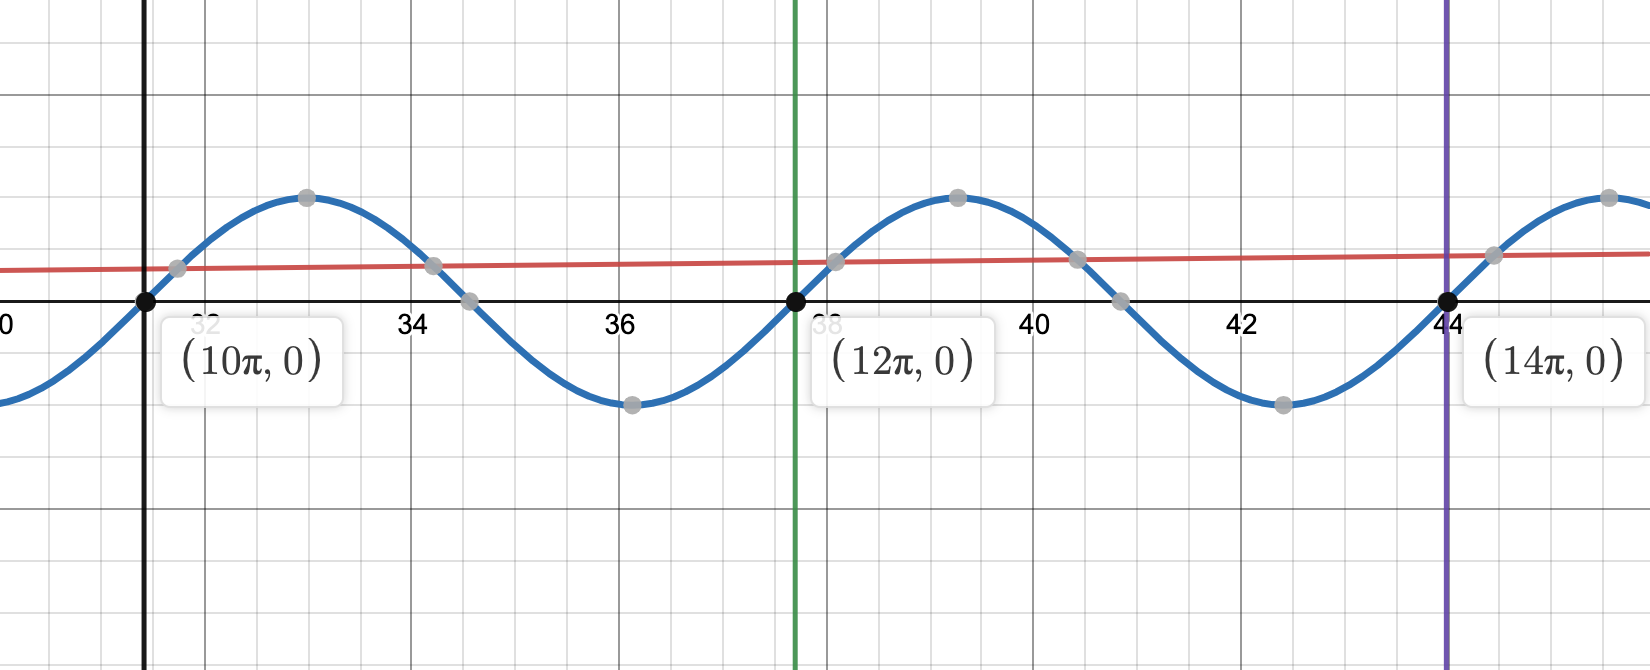
\includegraphics[width=12cm]{Intersections.png}
    \caption{$y=\frac{x}{100}$ having 2 intersections with $\sin{x}$ per period}
    \label{fig:my_label}
\end{figure}

\end{example}




\vspace{5mm}
\begin{example}
\begin{problem}[ARML 2021 T-4]
Compute the number of real values of $x$ such that $\cos(\cos(x))=\frac x{10}$.
\end{problem}

\vspace{5mm}
\noindent Without a graphing calculator, cos(cos(x)) is not the easiest to graph. It is possible, and we'll go over this later, but as of right now, we'll have to approach this problem a different way. If you take the $\arccos$ of both sides, we get $\cos(x) = \arccos(\frac{x}{10})$. Now, we'll have to graph both functions and find where they intersect.

\vspace{5mm}
\noindent Remember that even though we have $\arccos(\frac{x}{10})$, the real equation is $\cos(y)=\frac{x}{10}$ and that $\arccos$ only has a range from 0 to 1. $\cos$ can go from -1 to 1, so we have to graph both $\arccos(\frac{x}{10})$ and $-\arccos(\frac{x}{10})$. We know that $\arccos$ is 0 at $x=10$ and $\frac{\pi}{2}$ at $x=0$. Then, draw a line between these two points. The graph isn't an actual line, but we know that the x10 scaling factor makes $\arccos$ "basically" a line. Graphing the intersections gets a final answer of $\boxed{3}$.

\begin{figure}[H]
    \centering
    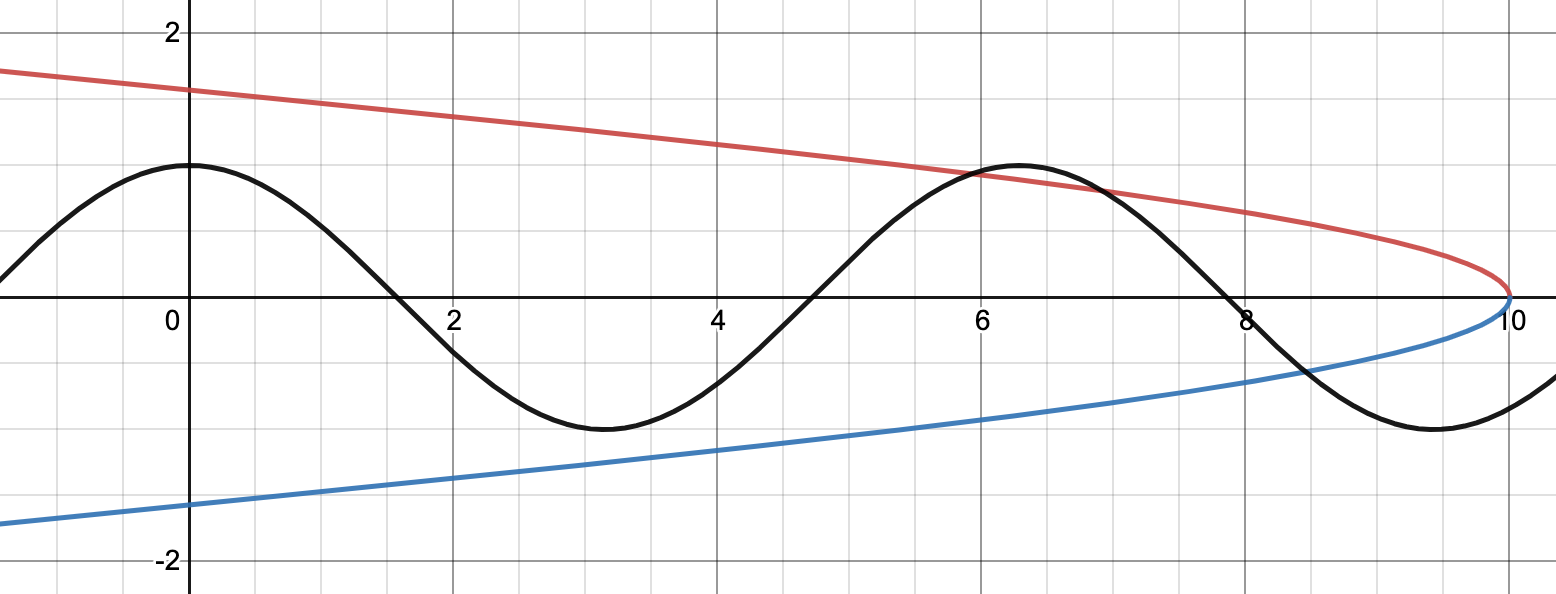
\includegraphics[width=12cm]{Intersections2.png}
    \caption{The 3 intersections}
    \label{fig:my_label}
\end{figure}

\end{example}

%\pagebreak
% \subsection{Trig Function Composition}
% \begin{example}
% \begin{problem}
% Find


% \end{problem}
% \end{example}

% \begin{example}
% \begin{problem}
% Find the period of $\cos(\cos(x))$
% \end{problem}

% \vspace{5mm}
% Try plugging in values. $x=0$ does not help because we don't know $\cos(1)$. If we plug in $x=\frac{\pi}{2}$, we get 1. This repeats every odd multiple of $\frac{\pi}{2}$; thus the period is $\boxed{\pi}$.

% \end{example}

\section{Hyperbolic Trig}
Not real trig.


\end{document}
